\documentclass[runningheads]{llncs}
\usepackage[T1]{fontenc}
\usepackage{booktabs,array,graphicx}
\usepackage{flafter}
\usepackage{hyperref}
\usepackage{url}
\hypersetup{hidelinks}
\emergencystretch=2em
\newcommand{\code}[1]{\texttt{#1}}
% Generated from validated signoff bundles.
\newcommand{\DesignCount}{7}
\newcommand{\StageCount}{21}
\newcommand{\TestPasses}{955}
\newcommand{\TestSkipped}{15}
\newcommand{\CellMin}{16}
\newcommand{\CellMax}{1024}
\newcommand{\SetupMin}{4.911}
\newcommand{\HoldMin}{0.049}
\newcommand{\RuleCount}{211}
\newcommand{\ModelCalls}{1}
\newcommand{\ModelInputTokens}{6999}
\newcommand{\ModelOutputTokens}{1403}
\newcommand{\SourceShort}{af31b39f6782}
\newcommand{\InitialAluDRC}{1}
\newcommand{\PaddingBefore}{0}
\newcommand{\PaddingAfter}{2}
\newcommand{\ClockPeriod}{10.0}
\newcommand{\ClockUncertainty}{0.25}
\newcommand{\OutputLoad}{0.05}
\newcommand{\RepairRuntime}{168.8}
\newcommand{\RepairModel}{claude-sonnet-5}

% Generated from native attack, repair and repeat evidence.
\newcommand{\NativeAttackTrials}{18}
\newcommand{\NativeBlocked}{18}
\newcommand{\NativeFalseClean}{18}
\newcommand{\DegradedRuleCount}{152}
\newcommand{\StudyEpisodes}{9}
\newcommand{\StudyVerified}{7}
\newcommand{\StudyEscalated}{2}
\newcommand{\StudySuccessPct}{77.8}
\newcommand{\StudyEscalationPct}{22.2}
\newcommand{\StudyModelCalls}{20}
\newcommand{\StudyInputTokens}{174306}
\newcommand{\StudyOutputTokens}{50164}
\newcommand{\ProposalPromotions}{20}
\newcommand{\ConfirmedBadProposals}{11}
\newcommand{\UncheckedProposals}{2}
\newcommand{\TimingBefore}{-0.326192}
\newcommand{\TimingAfter}{0.001586}
\newcommand{\CounterStressWNS}{-0.715689}
\newcommand{\LargeCells}{1024}
\newcommand{\RepairSourceShort}{18d948815ac6}
\newcommand{\ExactRoutePairs}{6}
\newcommand{\NormalizedGDSPairs}{6}

\title{Candidate-Bound Evidence for RTL-to-GDS Signoff: An Open-Source Orchestration Study}
\titlerunning{Candidate-Bound Signoff and Verified Repair}
\author{Rithwik Vallabhan TV \and Sreejeesh SG \and Jayaraj U Kidav \and Nanditha N Varma}
\authorrunning{R. Vallabhan TV et al.}
\institute{NIELIT Calicut, India\\
\email{rithwik@calicut.nielit.in, sreejeesh@nielit.gov.in}\\
\email{jayaraj@nielit.gov.in, nanditha@calicut.nielit.in}}
\begin{document}
\maketitle
\begin{abstract}
A clean physical-verification report is useful only if its checks cover the
implementation selected for release. RTL2GDSAGI binds RTL, constraints,
layout, parasitics, verification inputs, and native gate records to a candidate
manifest and revalidates these identities before local signoff. We evaluate
\DesignCount\ SKY130 designs spanning \CellMin--\CellMax\ mapped cells and
complete the declared \StageCount-stage contract, including synthesis and
routed equivalence, extracted-parasitic timing, DRC, LVS, and antenna checks.
A native fault-injection study covers six stale or incomplete evidence classes,
with three replicates each. A comparator based on successful exit or cached
status accepts all \NativeAttackTrials\ fixtures; the candidate-aware checks
block all \NativeBlocked\ cases. Nine live model-assisted repair trials cover
spacing, power-network construction, and stressed setup timing; \StudyVerified\
complete full rechecking and \StudyEscalated\ escalate. At an unchanged 3 ns
period, one ALU repair improves setup slack from \TimingBefore\ ns to
\TimingAfter\ ns. Repeated implementation runs produce \ExactRoutePairs\
identical routed-DEF pairs and \NormalizedGDSPairs\ identical GDS pairs after
zeroing timestamp payloads; raw GDS hashes and candidate identifiers can
differ. All tables are generated from retained native artifacts and audit logs.
\keywords{RTL-to-GDS \and physical verification \and artifact provenance
\and electronic design automation \and verified repair}
\end{abstract}

\section{Introduction}
OpenROAD and OpenLane provide practical open infrastructure for synthesis and
physical implementation~\cite{ajayi2019,shalan2020}. Their native checks answer
different questions: timing concerns a constrained circuit and parasitic
network; DRC concerns geometry under a rule deck; and LVS concerns the layout
and its schematic reference. A controller must establish that these answers
support the same release candidate. Zero DRC markers can accompany a stale
layout or an incomplete rule inventory, and a success message can appear
without a real LVS comparison. Repairs create an additional opportunity for
previously valid evidence to become stale.

RTL2GDSAGI is a Python controller that combines native tool execution with
content-bound gate evidence. A model proposes a configuration change;
deterministic code authorizes the changed surface and requires the affected
native checks before promotion. This paper tests three questions: whether
these checks reject specific false-clean fixtures, whether live repairs survive
native rechecking, and which implementation artifacts reproduce across runs.

The contributions are an executable candidate and gate contract, a native
fault study that isolates six false-clean conditions, and a measured repair
study with a comparator that accepts proposals without rechecking. The
underlying synthesis, placement, routing, and verification algorithms come
from the selected EDA tools. We claim detection of the tested fault classes;
we do not claim that provenance alone establishes manufacturing qualification
or that other controllers cannot implement comparable contracts.

\section{Candidate and Gate Contract}
\subsection{Execution and content identity}
The \StageCount\ stages are characterization, lint, simulation, constraint
generation, synthesis, synthesis equivalence, pre-layout timing, floorplan,
power-network generation, placement, clock-tree synthesis, post-CTS timing,
routing, extraction, post-route timing, GDS stream-out, DRC, LVS, antenna,
routed equivalence, and signoff. Pre-layout timing is advisory; post-CTS timing
gates hold slack, and post-route timing gates both setup and hold. Signoff
requires every declared hard obligation to be supported by positive evidence.

Verilator and Icarus Verilog provide lint and self-checking simulation. Yosys
and EQY provide synthesis and equivalence~\cite{eqydocs}. OpenROAD provides
physical implementation, extraction, and physical-stage timing. KLayout
streams and verifies the layout. The artifact ledger records a producer,
size, path, and SHA-256 digest for each output. Directory identities hash
relative filenames and file contents. The candidate manifest additionally
records configuration, constraints, selected PDK identity, and tool identities.
The layer map and DRC/LVS decks are bound inputs because their contents change
the meaning of the verification results.

Writing $H$ for SHA-256, the candidate identity is
\begin{equation}
 C=H\!\left(T,\{(k,H(A_k))\}_{k\in B},P,V,H(K),H(I)\right),
\end{equation}
where $T$ is the top, $B$ the bound artifact keys, $P$ the selected PDK identity,
$V$ the recorded tool identities, $K$ the run configuration, and $I$ the typed
configuration state. The PDK identity includes its name, root, standard-cell
library, and corner; it is not a hash of every file in the PDK installation.
Verification decks and the stream-out map are hashed as members of $B$.

Each gate declares its consumed and produced artifact keys, report key, parser
contract, and accepted tool identity. Release revalidation rehashes the files,
checks gate lineage, and checks that DRC and LVS consumed the selected GDS.
A certification identifier commits to the candidate identifier and gate records.
The native KLayout invocation is also checked against the selected input and
deck bytes, so an argument that selects another clean file is rejected.
Figure~\ref{fig:architecture} shows this boundary.

\begin{figure}[htbp]
\centering\small
\begin{tabular}{@{}c@{\quad}c@{\quad}c@{}}
\fbox{\parbox[c][0.9cm][c]{0.26\linewidth}{\centering RTL, tests,\\constraints, PDK}}
& $\longrightarrow$ &
\fbox{\parbox[c][0.9cm][c]{0.43\linewidth}{\centering Native execution\\and deterministic checking}}\\[5pt]
& & $\downarrow$\\[5pt]
\fbox{\parbox[c][0.9cm][c]{0.26\linewidth}{\centering Rehash and lineage\\check before release}}
& $\longleftarrow$ &
\fbox{\parbox[c][0.9cm][c]{0.43\linewidth}{\centering Candidate manifest\\and gate evidence}}\\[8pt]
\multicolumn{3}{c}{Failure $\rightarrow$ model proposal $\rightarrow$ authorization $\rightarrow$ native rechecking}
\end{tabular}
\caption{The model proposes changes; the controller evaluates native evidence
and candidate identity before promotion.}\label{fig:architecture}
\end{figure}

\subsection{Required native evidence}
DRC requires a usable report, the expected top, and the approved rule inventory
under the exact deck identity. The selected runset has \RuleCount\ normalized
active categories; 213 raw declarations include two narrowly approved aliases.
A zero-marker report with missing categories is insufficient. LVS requires
agreement among exit status, log verdict, and a native database containing
actual circuit cross-references. Its deck must contain an executable comparison
and belong to the approved set. Stream-out checks nonempty geometry, resolved
references, and layer numbers compatible with the PDK mapping. The PDN check
requires supply nets, follow-pin rails, straps, and vertical via connections.
These are structural obligations; IR drop and electromigration are outside
the implemented contract.

Extraction compares the logical net identities in SPEF and routed DEF, rejects
missing or duplicate nets, and requires complete parasitic sections. Standard
punctuation escapes are decoded before comparing hierarchical names. Native
signoff STA separately requires zero unannotated and partially unannotated
drivers and finite setup and hold slack meeting the fixed guardband. The model
cannot change clock period, uncertainty, output load, or verification decks.

\subsection{Repair and equivalence}
The Anthropic response schema distinguishes scalar configuration actions from
exact RTL text patches. The safety checker limits writable fields according
to the deterministic failure class and selects the earliest affected stage.
A physical change invalidates downstream artifacts and evidence. Native
rechecking must cover the action-derived obligations before the change becomes
a verified repair; a model confidence value does not determine acceptance.

EQY partition cuts can make related outputs independent even when they feed
joint next-state logic. The controller splits vector nets into scalar matches and groups the matched
signals to prove their joint relation. Counter and shift-register controls pass this configuration;
a control forcing a mapped counter-flop input to zero produces a counterexample.
A later successful strategy resolves an earlier unknown only for the same
partition, while a counterexample or unresolved terminal result blocks release.
This is a correction to proof decomposition, not a new equivalence algorithm.

\section{Experimental Protocol}
\subsection{Designs and environment}
The design set contains a register, registered multiplexer, eight-bit ALU,
counter, bidirectional shift register, four-entry FIFO, and a 1,024-stage
serial shift register. The latter supplies a larger synthetic case with
\LargeCells\ mapped cells; it extends scale rather than adding an independent
application domain. Each design has an authoritative self-checking testbench.

The PDK is SKY130A at Volare revision \code{bdc9412b3e46}.
We use the HD cell library at its typical 25\,$^{\circ}$C, 1.8 V corner
(\code{tt\_025C\_1v80}). The native container uses OpenROAD commit
\code{41a51eaf4ca2} and KLayout 0.28.2; native pre-layout
OpenSTA reports version 3.1.0. Baseline constraints use \ClockPeriod\ ns,
\ClockUncertainty\ ns uncertainty, and \OutputLoad\ pF output load. The
stressed ALU uses 3 ns with the same uncertainty and load. Physical parameters
and complete commands are retained in each run.

The paired baseline flows use source fingerprint \code{\SourceShort}; the
nine live repair episodes use the archived repair-cohort snapshot
\code{\RepairSourceShort}. Both snapshots and exact commands are retained.
The larger shift register uses two placement-padding sites, 25\% core
utilization, 0.35 placement density, an 80\% conservative antenna prediction
margin, eight native antenna repair iterations, eight routing workers, and
passive filler cells. These settings change implementation and repair effort;
the final antenna gate retains the original rule limits. Native antenna
checking remains mandatory even when global-route repair predicts no violations.

We run each selected design twice from RTL through signoff. Concurrent jobs
make elapsed time an observation of this environment, including container
overhead, rather than an isolated performance comparison. A separate
extractor validates candidate hashes, gate contracts, lineage, and certification
identity before generating the tables. Cell area comes from the synthesis
library report; die area comes from routed DEF coordinates and database units.

\subsection{Native fault injection and comparators}
The six fault classes in Table~\ref{tab:faults} use three replicates each.
Stale-input trials run native DRC on a physically different, clean ALU layout
with the same top name, while the candidate selects the current ALU layout.
The rule-coverage trials disable FEOL checks in a copy of the real DRC deck.
The LVS fixture writes a database-shaped file and prints a match without
calling compare. The layer-map fixture performs a real stream-out with the
mapping assignment omitted, then runs native DRC. PDN fixtures remove via
connections from a retained DEF. The final fixture substitutes a foreign GDS
after a verified ALU repair while retaining the repair's DRC/LVS records.

The comparator accepts zero DRC markers after successful exit, an LVS match
message after successful exit, or retained green status with a nonempty
artifact for the cached PDN and post-repair cases. It deliberately omits
coverage and candidate-identity checks. This controlled comparator isolates
the verification obligation; it is not a measured implementation of OpenLane,
ORFS-Agent, or another named external controller. Stale-input repetitions use
the same two ALU candidates. Other fixtures span register, ALU, and FIFO
candidates or three distinct foreign layouts, as recorded in the evidence.

\subsection{Live repair study}
Three repeats are declared for each of three injected failures: unpadded ALU
spacing, an excessive register PDN strap offset of 50~$\mu$m, and ALU setup
failure at 3 ns. Each episode uses Claude Sonnet 5 (Anthropic API; identifier
\code{claude-sonnet-5}), automatic typed authorization, and the recorded retry
policy. Every declared episode remains in the denominator. Model proposals
can differ between repeats, and native tools determine the recheck outcomes.

A second comparator retrospectively replays the same authorized proposals,
labeling each as promoted without repeating native checks. Native outcomes
are used only to assess whether that promotion was supported.
We evaluate this comparator at the proposal level,
separately from the episode outcome. A native failed recheck establishes a
confirmed false-clean promotion; an unavailable required recheck establishes
an unsupported promotion. Earlier development and provider-transport failures
are tabulated separately in the supplementary live-episode catalog.

\section{Results}
\begin{table}[htbp]\centering\small\setlength{\tabcolsep}{4pt}
\caption{Measured implementation results. Cell area is the synthesis-library area; die area comes from routed DEF. Timing uses extracted parasitics.}\label{tab:qor}
\begin{tabular}{@{}lrrrrr@{}}\toprule
Design & Cells & Cell area & Die area & Setup slack & Hold slack \\
 & & ($\mu$m$^2$) & ($\mu$m$^2$) & (ns) & (ns) \\
\midrule
register & 22 & 292.78 & 2393.17 & 6.954 & 1.204 \\
mux4to1 & 48 & 480.46 & 3602.40 & 6.952 & 1.203 \\
alu8 & 133 & 1018.48 & 6125.41 & 5.256 & 1.192 \\
counter & 47 & 416.65 & 3279.28 & 4.911 & 0.494 \\
shift\_reg & 16 & 380.36 & 3091.92 & 6.892 & 0.554 \\
fifo\_buf & 109 & 1721.65 & 9169.02 & 6.396 & 0.273 \\
shift1024 & 1024 & 25624.58 & 115705.42 & 5.553 & 0.049 \\
\bottomrule\end{tabular}\end{table}

\begin{table}[htbp]\centering\small\setlength{\tabcolsep}{4pt}
\caption{Native verification and execution outcomes. Every design passed all 21 stages, both equivalence boundaries, LVS, and its authoritative testbench.}\label{tab:gates}
\begin{tabular}{@{}lrrrrr@{}}\toprule
Design & Route/DRC & Antenna & SPEF nets & GDS & Runtime \\
 & violations & net/pin & & (KiB) & (s) \\
\midrule
register & 0/0 & 0/0 & 35 & 131.8 & 31.7 \\
mux4to1 & 0/0 & 0/0 & 87 & 161.6 & 45.8 \\
alu8 & 0/0 & 0/0 & 157 & 497.2 & 73.1 \\
counter & 0/0 & 0/0 & 62 & 238.4 & 36.5 \\
shift\_reg & 0/0 & 0/0 & 32 & 117.4 & 32.4 \\
fifo\_buf & 0/0 & 0/0 & 126 & 486.6 & 54.4 \\
shift1024 & 0/0 & 0/0 & 1210 & 3309.2 & 145.6 \\
\bottomrule\end{tabular}\end{table}

\subsection{Implementation and verification}
All \DesignCount\ selected designs complete \StageCount/\StageCount\ stages
with clean local certification. Table~\ref{tab:qor} reports mapped size, area,
and extracted-parasitic timing. Detailed routing and DRC each report zero
violations. Every DRC report contains the approved \RuleCount-category
inventory. Native LVS matches; antenna checking reports zero violating nets
and pins; and synthesis and routed equivalence pass. Every supplied testbench
passes, and each SPEF covers every routed signal net counted by the identity
check. Table~\ref{tab:gates} retains physical and runtime measurements.

\subsection{False-clean evidence}
\begin{table}[htbp]\centering\small\setlength{\tabcolsep}{4pt}
\caption{Native fault fixtures and the controlled status/count comparator. Replicates are defined in the protocol.}\label{tab:faults}
\begin{tabular}{@{}p{0.25\linewidth}p{0.37\linewidth}rr@{}}\toprule
Fixture & Observed evidence & Naive clean & Blocked \\
\midrule
Stale same-top GDS & DRC 0; input mismatch & 3/3 & 3/3 \\
Missing FEOL rules & DRC 0; 152 categories & 3/3 & 3/3 \\
LVS without compare & Match; zero cross-refs & 3/3 & 3/3 \\
Missing PDN connections & Nonempty DEF; zero vias & 3/3 & 3/3 \\
Missing layer map & DRC 0; invalid layer shapes & 3/3 & 3/3 \\
GDS swap after repair & Cached pass; digest mismatch & 3/3 & 3/3 \\
\bottomrule\end{tabular}\end{table}

The comparator accepts \NativeFalseClean/\NativeAttackTrials\ fault fixtures;
the implemented checks reject \NativeBlocked/\NativeAttackTrials. Disabling
FEOL produces zero markers but only \DegradedRuleCount\ normalized categories.
Omitting the layer map also produces a native zero-marker result, while the
stream-out check finds routing shapes on incompatible layer numbers. The fake
LVS database has zero circuit cross-references despite its match message.
These results show why content identity, rule coverage, and comparison evidence
are separate requirements. They establish detection of the six tested classes,
not completeness against arbitrary checker or host compromise.

\subsection{Live repair and timing stress}
\begin{table}[htbp]\centering\small\setlength{\tabcolsep}{4pt}
\caption{All declared live repair episodes. Verified means the complete native signoff contract passed.}\label{tab:repairs}
\begin{tabular}{@{}lrrrr@{}}\toprule
Injected failure & Trials & Verified & Escalated & Calls \\
\midrule
Spacing: padding 0 & 3 & 3 & 0 & 3 \\
PDN: offset 50 $\mu$m & 3 & 3 & 0 & 3 \\
Setup: period 3 ns & 3 & 1 & 2 & 14 \\
\bottomrule\end{tabular}\end{table}

Of \StudyEpisodes\ declared episodes, \StudyVerified\ reach full verification
(\StudySuccessPct\%) and \StudyEscalated\ escalate (\StudyEscalationPct\%).
Spacing and PDN construction each succeed in three repeats; stressed timing
succeeds in one of three. These are descriptive results on repeated fixtures,
not a population repair-success estimate. The cohort makes \StudyModelCalls\
provider calls, with \StudyInputTokens\ input and \StudyOutputTokens\ output
tokens. Token counts are provider observations, not inferred cost estimates.

All three stressed ALU trials initially reach routed setup WNS
\TimingBefore\ ns under a generated 3.000 ns SDC period. In the successful
trial, the delay-oriented mapping first remains negative; a subsequent
placement update reaches \TimingAfter\ ns with unchanged clock and protected
RTL. The resulting layout passes all downstream checks. The small positive
margin is a result at the stated typical corner and guardband, not evidence
of multi-corner closure. A separate counter control at an unchanged 1.5 ns
period reaches setup WNS \CounterStressWNS\ ns and is blocked by the native
timing gate. Figure~\ref{fig:stress} shows the measured ALU recheck sequence.

\begin{figure}[htbp]\centering
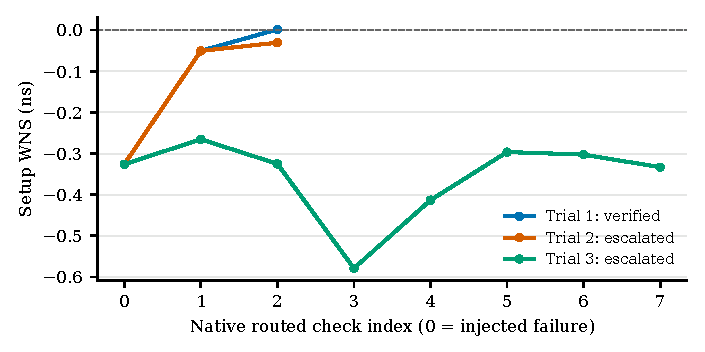
\includegraphics[width=0.95\linewidth]{figures/timing_stress.pdf}
\caption{Native routed setup checks at the unchanged 3 ns period. Lines end
at the last completed routed check; the legend gives each episode's terminal
outcome.}
\label{fig:stress}\end{figure}

The comparator that skips rechecking promotes \ProposalPromotions\ authorized
proposals. Native rechecks show \ConfirmedBadProposals\ confirmed failures;
\UncheckedProposals\ additional promotions lack a completed required target
check. The production controller does not certify those proposal states.
This result directly tests the danger of accepting a model's change as its own
verification evidence. The earlier live episodes, including malformed
responses and authentication/grammar failures, remain visible in the catalog.

\subsection{Repeated artifacts and regressions}
\begin{table}[htbp]\centering\small\setlength{\tabcolsep}{4pt}
\caption{Seven frozen primary pairs. Date normalization zeros only BGNLIB/BGNSTR payloads; all other GDS bytes remain unchanged. Both netlists also match in every pair.}\label{tab:reproducibility}
\begin{tabular}{@{}lllll@{}}\toprule
Design & Routed DEF & SPEF & Raw GDS & Dates zeroed \\
\midrule
register & Same & Same & Same & Same \\
mux4to1 & Same & Same & Different & Same \\
alu8 & Same & Same & Different & Same \\
counter & Same & Same & Different & Same \\
shift\_reg & Same & Same & Different & Same \\
fifo\_buf & Same & Same & Different & Same \\
shift1024 & Same & Same & Different & Same \\
\bottomrule\end{tabular}\end{table}

The repeat comparison in Table~\ref{tab:reproducibility} uses content hashes.
Routed DEF, mapped and routed netlists, and SPEF reproduce exactly for
\ExactRoutePairs\ design pairs. Timestamp-neutral GDS hashes reproduce for
\NormalizedGDSPairs\ pairs after zeroing only BGNLIB and BGNSTR date fields.
All raw GDS hashes differ; some LVS serialization hashes also differ. The
larger pair selects different native li1-to-met1 via variants, changing DEF
and GDS bytes while mapped/routed netlists and SPEF remain identical.
Eight routing workers were used for this case; the cause of the variant
selection difference was not isolated. Candidate identifiers
therefore identify actual artifact bytes rather than a normalized geometry
class. Path-bearing characterization records can also differ between run
directories. We claim reproducibility at the explicitly reported levels; full
bitwise identity of every run file is not established.

The final regression suite reports \TestPasses\ passes, zero failures and
errors, and \TestSkipped\ skips. Skipped archived fixtures are not counted as
passed verification. The supplementary record preserves incomplete scale
probes including the 1,995-cell accumulator's spacing, antenna and diode-legalization
failures and the ALU-bank antenna failures. These failed runs are excluded from the clean-design count.

\section{Related Work}
OpenROAD and OpenLane supply the implementation infrastructure
~\cite{ajayi2019,shalan2020}. METRICS2.1 provides structured flow measurement
and tuning~\cite{jung2021}; PROV provides general provenance relationships
~\cite{prov2013}. ChatEDA studies LLM-based task decomposition, script
construction, and EDA execution~\cite{chateda}. ORFS-Agent studies iterative
parameter optimization in OpenROAD-flow-scripts~\cite{orfsagent}. MCP4EDA
connects language-model interaction to a complete tool flow and uses backend
feedback for synthesis optimization~\cite{mcp4eda}. FlowFixer-EDA describes
log-grounded diagnosis, patch validation, and native tool feedback for repair
~\cite{flowfixer}. These works establish that tool use and verified feedback
already form part of LLM-assisted EDA research. EDAid uses multiple
model-controlled agents to improve EDA workflow execution~\cite{edaid},
extending the comparison beyond single-agent controllers. AuDoPEDA evaluates
repository-grounded coding agents through executable OpenROAD changes and
measured quality of results~\cite{audopeda}.

ChiBench supplies a curated RTL corpus for testing EDA tools
~\cite{chibench}. DRVerify addresses physical-verification runset testing with
known legal and violating layout structures~\cite{drverify}. Such work
reinforces that a zero-marker count does not by itself establish rule intent
or coverage. EQY supplies the equivalence engine used here~\cite{eqydocs}.
The contribution of this study is the measured combination of native
false-clean fixtures, candidate-content lineage, and action-derived rechecking.
We make no unsupported priority claim that prior flows lack equivalent
protections. A comparative claim against another controller would require a
shared design set, tool environment, constraints, and verification obligations.

\section{Discussion and Limitations}
The fault fixtures demonstrate actual native false-pass outputs under the
specified weak comparators. The guard rejects them through several mechanisms:
input identity for stale GDS, approved inventory for missing rules, native
comparison evidence for fake LVS, structural connectivity for PDN, and layer
mapping for stream-out. Hashes preserve identity under a trusted controller,
host, tools, and PDK. They do not prove that an approved rule deck implements
every foundry requirement or that tool code and gate records cannot be forged.

The repair study contains only three fixture types and three repeats per type.
Its \StudyVerified/\StudyEpisodes\ outcome should not be generalized to unseen circuits or failure
classes. The larger shift register is a regular synthetic circuit; full camera,
processor, SRAM-macro, and multi-clock systems remain outside this evaluation.
The declared local signoff omits multi-corner timing, on-chip variation,
electrical power integrity, and foundry qualification. Formal equivalence
establishes preservation of the RTL relation, while simulation checks the
supplied behavioral tests rather than an external specification.
The JSONL audit retains every accepted proposal, native recheck metric, and
provider call count. Rollback can reuse a numbered attempt filename, so a
complete raw prompt--response and intermediate-artifact archive for every
proposal is not established. Final native artifacts and the cohort denominator
are retained.

\section{Conclusion}
RTL2GDSAGI binds native verification evidence to a selected implementation and
requires native rechecking of authorized model proposals. The measured flow
completes \DesignCount\ designs, including a \LargeCells-cell synthetic shift register.
All \NativeAttackTrials\ native false-clean fixtures are blocked. Of
\StudyEpisodes\ live repair episodes, \StudyVerified\ complete signoff and
\StudyEscalated\ escalate; the stressed ALU result preserves the 3 ns constraint.
Repeated artifacts reproduce at the stated content and timestamp-normalized
levels. The evidence supports the tested release contract and identifies the
remaining limits on larger applications and verification coverage.

\section*{Code, data, and AI assistance}
The public repository is \url{https://github.com/xp4t/rtl2gdsagi}. The versioned
paper artifact is available at
\url{https://github.com/xp4t/rtl2gdsagi/releases/tag/rtl2gdsagi-paper-20261012}.
It includes source snapshots, exact commands, native reports, content digests,
all retained live repair episodes, and scripts that regenerate the tables.
The repair study uses Claude Sonnet 5 from Anthropic. Codex assisted writing
and three final internal review passes addressing evidence, methods/citations, and
final presentation. These passes share the same conversational context and
are not independent external peer review.

\appendix
\section{Repair Episodes and Incomplete Scale Probes}
Table~\ref{tab:episodes} lists each declared episode. Earlier live API episodes
appear in Table~\ref{tab:history}; the supplemental JSON catalog maps each row
to its retained run path and error records. They are not pooled into the nine
episodes because action schemas and provider transport changed during
development. Interrupted scale probes, DRC failures, and antenna failures are
retained with their measured stage outcomes and are excluded from the completed
design count. Clock-buffer discovery, path handling, and terminal-verdict
parsing are implementation prerequisites rather than independent contributions.
\begin{table}[htbp]\centering\small\setlength{\tabcolsep}{4pt}
\caption{All nine original live repair episodes on source 18d948815ac6. These archived outcomes are separate from frozen replay and larger episodes.}\label{tab:episodes}
\begin{tabular}{@{}lllll@{}}\toprule
Episode & Initial failure & Final evidence & Calls & Outcome \\
\midrule
Spacing 1 & 1 marker & Full signoff & 1 & Verified \\
Spacing 2 & 1 marker & Full signoff & 1 & Verified \\
Spacing 3 & 1 marker & Full signoff & 1 & Verified \\
PDN 1 & PDN-0185 & Full signoff & 1 & Verified \\
PDN 2 & PDN-0185 & Full signoff & 1 & Verified \\
PDN 3 & PDN-0185 & Full signoff & 1 & Verified \\
Setup 1 & -0.326192 ns & 0.001586 ns & 2 & Verified \\
Setup 2 & -0.326192 ns & Not certified & 3 & Escalated \\
Setup 3 & -0.326192 ns & Not certified & 9 & Escalated \\
\bottomrule\end{tabular}\end{table}

\begin{table}[htbp]\centering\small\setlength{\tabcolsep}{4pt}
\caption{All retained earlier live API episodes. API errors include authentication, transport and response validation. The catalog preserves their distinct protocols.}\label{tab:history}
\begin{tabular}{@{}llrl@{}}\toprule
Case & First requested stage & Responses & Outcome \\
\midrule
H1 & drc & 1 & Verified \\
H2 & drc & 0 & Stopped; API error \\
H3 & drc & 1 & Verified \\
H4 & drc & 1 & Verified \\
H5 & sta\_signoff & 0 & Stopped; API error \\
H6 & sta\_signoff & 0 & Stopped; API error \\
H7 & sta\_signoff & 1 & Stopped; action rejected \\
H8 & sta\_signoff & 0 & Stopped; API error \\
H9 & lint & 0 & Stopped; API error \\
H10 & lint & 1 & Stopped; API error \\
\bottomrule\end{tabular}\end{table}


\begin{thebibliography}{13}
\bibitem{ajayi2019}
Ajayi, T., et al.: Toward an Open-Source Digital Flow. In: Proceedings of the 56th Annual Design Automation
Conference (2019). \url{https://doi.org/10.1145/3316781.3326334}
\bibitem{jung2021}
Jung, J., Kahng, A.B., Kim, S., Varadarajan, R.: METRICS2.1 and flow tuning
in the IEEE CEDA Robust Design Flow and OpenROAD: ICCAD special session paper.
In: Proceedings of the 2021 IEEE/ACM International Conference on Computer-Aided
Design (2021). \url{https://doi.org/10.1109/ICCAD51958.2021.9643541}
\bibitem{shalan2020}
Shalan, M., Edwards, T.: Building OpenLANE: A 130nm OpenROAD-based
tapeout-proven flow. In: Proceedings of the 2020 IEEE/ACM International
Conference on Computer-Aided Design (2020).
\url{https://doi.org/10.1145/3400302.3415735}
\bibitem{prov2013}
W3C: PROV-Overview: An overview of the PROV family of documents.
W3C Working Group Note (2013). \url{https://www.w3.org/TR/prov-overview/}
\bibitem{eqydocs}
YosysHQ: EQY documentation. \url{https://yosyshq.readthedocs.io/projects/eqy/en/latest/}
(accessed 12 October 2026)
\bibitem{chateda}
Wu, H., He, Z., Zhang, X., Yao, X., Zheng, S., Zheng, H., Yu, B.:
ChatEDA: A Large Language Model Powered Autonomous Agent for EDA.
IEEE Transactions on Computer-Aided Design of Integrated Circuits and Systems
43(10), 3184--3197 (2024). \url{https://doi.org/10.1109/TCAD.2024.3383347}
\bibitem{orfsagent}
Ghose, A., Kahng, A.B., Kundu, S., Wang, Z.:
ORFS-Agent: Tool-Using Agents for Chip Design Optimization.
In: Proceedings of the ACM/IEEE International Symposium on Machine Learning
for CAD (2025). \url{https://doi.org/10.1109/MLCAD65511.2025.11189204}
\bibitem{mcp4eda}
Wang, Y., Ye, W., He, Y., Chen, Y., Qu, G., Li, A.:
MCP4EDA: LLM-Powered Model Context Protocol RTL-to-GDSII Automation with
Backend Aware Synthesis Optimization. arXiv:2507.19570 (2025).
\url{https://arxiv.org/abs/2507.19570}
\bibitem{flowfixer}
Dong, K., Wang, R., Yuan, F., An, B., Zhang, X.: FlowFixer-EDA: A Tool-Feedback-Augmented Large Language Model Agent for
Automated Diagnosis and Repair of Open-Source RTL-to-GDS Design Flow Failures.
IEEE Access 14, 140412--140428 (2026).
\url{https://doi.org/10.1109/ACCESS.2026.3730896}

\bibitem{chibench}
Sumitani, R., Amorim, J.V., Mafra, A., Crepalde, M., Pereira, F.M.Q.:
ChiBench: A Benchmark Suite for Testing Electronic Design Automation Tools.
arXiv:2406.06550 (2024). \url{https://arxiv.org/abs/2406.06550}
\bibitem{drverify}
Sage Design Automation: DRVerify: The Verification of Physical Verification.
Technical white paper (2018).
\url{https://semiwiki.com/wp-content/uploads/2018/06/sage_DRVerify_WP_v2-3-1.pdf}
\bibitem{edaid}
Wu, H., Zheng, H., He, Z., Yu, B.: Divergent Thoughts toward One Goal:
LLM-based Multi-Agent Collaboration System for Electronic Design Automation.
In: Proceedings of NAACL-HLT, vol. 1, pp. 1710--1721 (2025).
\url{https://doi.org/10.18653/v1/2025.naacl-long.83}
\bibitem{audopeda}
Ghose, A., Jang, J., Kahng, A.B., Lee, J.:
Automated QoR improvement in OpenROAD with coding agents.
arXiv:2601.06268v2 (2026). \url{https://arxiv.org/abs/2601.06268v2}
\end{thebibliography}
\end{document}
